\chapter{Analysis and Review}
In this chapter we will review the goals set out in chapter 3.3 Analysis and to what extent these have been achieved, where success was observed and where failures occured and what improvements could be made.
We will first review the metrics associated with the framework then with the use of the framework and finally we will review some output produced with our sample project.
\section{Metrics report}
\subsection{Framework - Reliability}
As there is no active use of the framework, the only viable data for reliability of the framework is our active development bug tracking, test coverage data and code scene analysis.
Framework test coverage is at \(95\%\) code coverage which is respectable.
There are no active bugs currently identified, and non-trivial code contains documentation.
\begin{figure}[h]
 \centering
 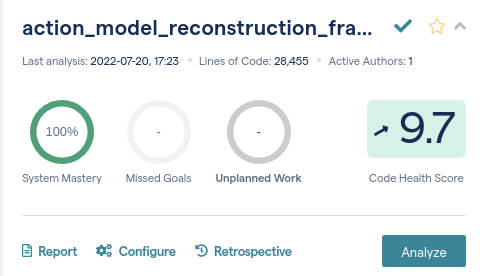
\includegraphics[width=0.7\textwidth]{images/code/Selection_062}
 \caption{Code health analysis Code Scene}
 \label{fig:code-health}
\end{figure}
Considering the 28,000 lines of code (including some patched work on open-source projects) a health score of 9.7 can be considered as excellent hence we are satisfied with the reliability.
\newpage
\subsection{Framework - Maintainability}
\begin{figure}[h]
 \centering
 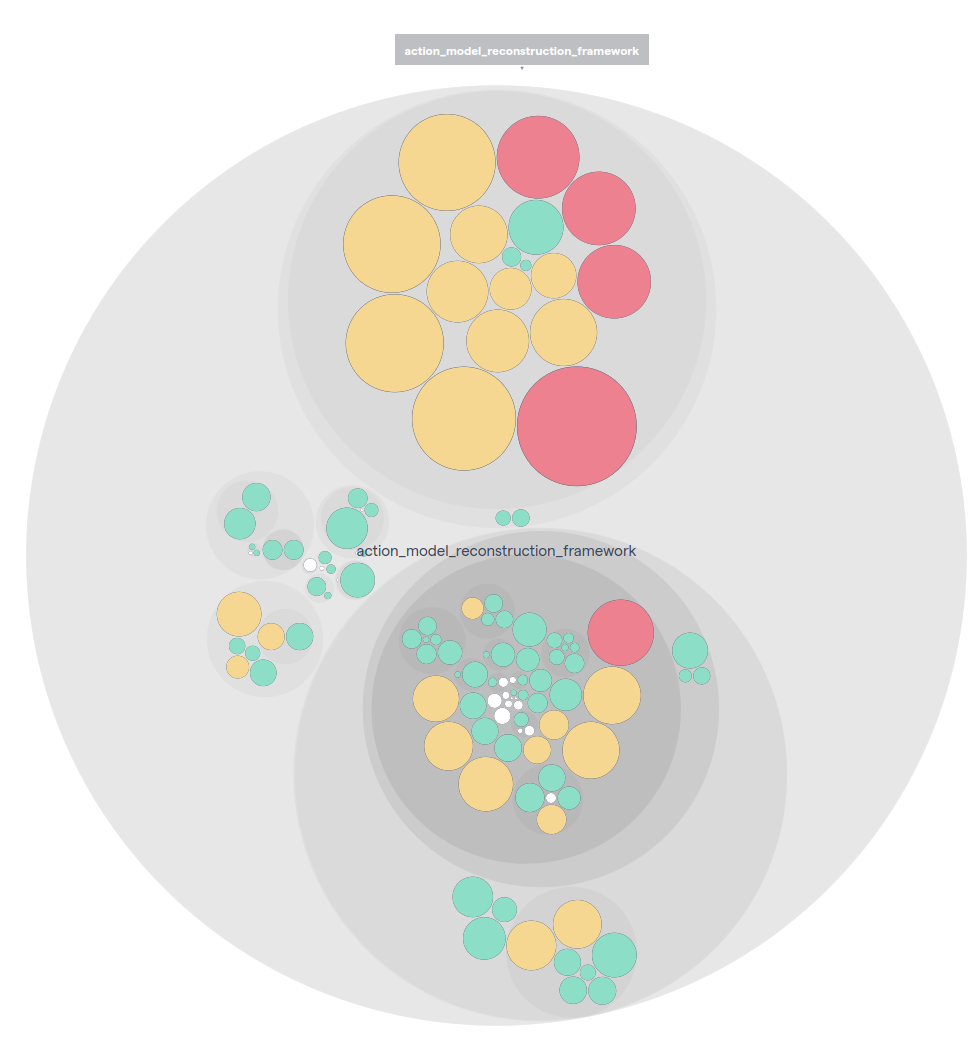
\includegraphics[width=0.7\textwidth]{images/code/hotspot}
 \caption{Code maintenance cost (green = low, red = high)}
 \label{fig:hotspots}
\end{figure}
Above is a code-hotspot visualisation meant to visualise the difficulty of maintaining the active code-base, each colored circle represents a file, whilst grey layers represent directories/modules.
The large circle in the top half contains the FFXSolver module, we can observe that the code bellow developed for the purpose of the framework is kept in a maintainable state (green).
This visualisation is generated using automated metrics for file and code complexity.
We can also observe that as stated, each module (simulator, learn, parser, generator) represented by the first layer of smaller light gray circles to the left, are kept completely isolated this is important as there should be no coupling between these.
It can be concluded that for the code associated with the framework, the maintenance cost is low.

\subsection{Framework - Testability}
As previously mentioned we have achieved \(95\%\) test coverage over all code for unit tests.
We have also included integration tests with the various open-source tools used such as the solvers and learning models.
For maintaining a high testing standards, we deployed a testing pipeline making use of github actions to ensure that new code is tested before being merged into the codebase.
Other functional tests such as smoke tests were not performed as these are simply not required at this stage.
If more users adopt the use of the repository then such tests will be adopted.
There are currently no seriously lacking forms of necessary tests.

\subsection{Framework - Portability}.
We have set a pipeline ensuring that functionality is supported across all major python versions from 3.6 onwards.
The pipeline also includes test execution on Linux, Windows and Mac OS to ensure the portability across these operating systems.

Portability to languages other than Python is non-existent as it is too early in the project to do so and the initial design specification justified the use of python as the primary language.

\subsection{Framework - Reusability}
As observed in figure\ref{fig:hotspots} the codebase is written with modularity in mind.
We have also demonstrated in our demo project that each module can be used independently for use-cases other than the ones we used them for.
We have further tested using the PDDL simulator separately for other projects to develop simple solving algorithms in python.
This presents a potential use-case for student's learning these topics to have access to the full power of PDDL and the simplicity of python when designing domains and solvers.

\subsection{User - Adoption friction}
The sample user project provided in chapter 4.3 code-snippet\ref{example-project} exemplifies the adoption friction a user will face when using our modules.
It is clear that working with PDDL and associated tools such as solvers is now much more straight forward as the only requirement is to have a domain file and a problem file to achieve functionality that was previously not possible.

\subsection{User - Learning curve}
We have kept the learning curve to a minimum.
In order to use the tools we have developed, a user must understand the basics of PDDL to be able to generate their own domain files, and problem files, as well as enough python to have a grasp of basic data structures.
A sample project and domain was created specifically for new users to get accustomed to the tools available.
We will expand these basic examples in the future in order to best demonstrate the available capabilities because we have not provided an online documentation page as of yet.
We are however lacking in comparison to more established projects as there is yet to be a public release on pypi for easier discovery.

\subsection{User - Development complexity}
Our demo project shows that no user-level files require high cyclomatic complexity (code branching factor) in the expected workflow.
We have also integrated the mccabe library to generate warning when complexity exceeds thresholds set by the PEP-8 standard by using the flake8 package in our workflow\cite{Flake8—f13:online}.
This is in line with modern frameworks, hence we can say it is a success.
The LOC count is also bellow 50 in all important integrations such as the DataGenarators or demo project files, which is important for reducing complexity and ensuring that the necessary functionality can be achieved efficiently with the available utility tools we provided.

\section{Sample project review}
In this section we will review the functionality we have provided and data we have produced with it.
As we stated, this demo project's goal is to train a set of Markov Logic Networks representing PDDL Actions in Python given a dataset that we synthetically engineer from any defined domain.

The first step is to generate a random dataset of problem files for our pddl domain so we can use their solutions as training data for the MLN.
From the frameworks generators module we have the following available domains from the IPC competition, more can be added following the specified rules:
\begin{figure}[h]
 \centering
 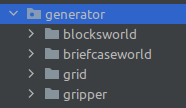
\includegraphics[width=0.4\textwidth]{images/code/generators}
 \caption{Integrated domains available for use}
 \label{fig:generators}
\end{figure}

To generate the necessary files for a domain such as Grid World, we can simply import the relevant generator and generate the problem files into our desired directory, flags for more or less complexity during generation can be specified.

\begin{lstlisting}[language=Python]
from generator.generator import GridWorldGenerator
GridWorldGenerator.generate_data(output_dir=PROBLEM_STATE_DSET_DIR)
\end{lstlisting}

The generated files are saved to the directory:
\begin{figure}[h]
 \centering
 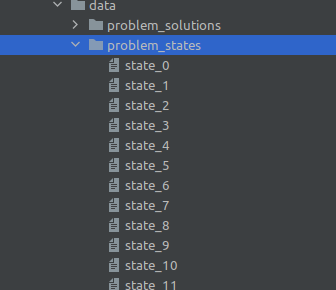
\includegraphics[width=0.4\textwidth]{images/code/problem_states}
 \caption{problem files generated}
 \label{fig:problem files}
\end{figure}

Similarly to how we generated problems, we can now generate solutions using one of the available solvers from our solving module:

\begin{lstlisting}[language=Python]
from solvers.solvers import FFXSolver
FFXSolver.solve_problem_dir(
    domain_file=DOMAIN_FILE,
    problem_dir=PROBLEM_STATE_DSET_DIR,
    output_dir=PROBLEM_SOLUTION_DIR,
)
\end{lstlisting}
This will generate one solution file for each problem in the directory specified.
Now that we have generated the necessary data to create our MLN dataset which relies on plan traces as opposed to simply plans without intermediate states, we can use the simulation module in order to execute a plan on the initial problem state:
\begin{lstlisting}[language=Python]
parsed = parse_pddl(domain_file)
problem = parse_state(f"{problem_state_dir}/state_{i}")
plan = parse_plan(f"{problem_solution_dir}/state_{i}")
state = State(parsed)
state.set_init_state(problem["init"])
for index, s in enumerate(plan["steps"]):
    p = Predicate(**s["predicate"])
    state.perform_action(p)
\end{lstlisting}

The above code is a simplified version in order to provide an indication of how a user can simulate a plan on an initial state.
For each sate and problem we generate an MLN database compatiblible with the learning module an abstraction is provided for simplicity:
\begin{lstlisting}[language=Python]
write_dbs(
    domain_file=DOMAIN_FILE,
    problem_state_dir=PROBLEM_STATE_DSET_DIR,
    problem_solution_dir=PROBLEM_SOLUTION_DIR,
    mln_db_path=MLN_DATABASE,
)
\end{lstlisting}

Finally we can train the model with the generated dataset:
\begin{lstlisting}[language=Python]
MLNDeclarationGenerator.gen(DOMAIN_FILE, DOMAIN_P_DECS)
model = PracmlnLearningModel(mln_database_path=MLN_DATABASE, domain_p_decs_path=DOMAIN_P_DECS)
model.train()
\end{lstlisting}

The above workflow demonstrates how straight forward it is to use each module.
We want to ensure that the way data is being manipulated, and managed is clear and concise, this is important because when users move towards gigabytes of data and thousands of files, any mistake can be extremely costly space-wise, computationally and time-wise for the user.
Complex algorithms such as PracmlnLearningModel are abstracted out by the developer/researcher of such models and a familiar interface is exposed to the user, now anyone can train a model in the Planning domain just as they would in the Machin Learning or Deep Learning domain.

\section{Evaluating trained model}
In this section we will evaluate the model we have trained.
To evaluate the model we track the change in weights for each predicate associated with an MLN representing an action in the domain.
If the value of a weight increases, then it means that the predicate has a higher likelihood of being applied in the action model.

We can test the robustness of the Network by applying noise (both systematic and random) to the database at different thresholds.
Systematic noise can be added by removing a target set of predicates with a given probability.
And Random noise can be added by removing any given predicate by a defined probability.

We measure accuracy by analysing how similar a derived logic network is to the expected logic network which we can construct. We can calculate the error rate for \(a_{pre}\) by the following formula:
\[E(a_{pre})=\frac{a_{pre}\cap \{p\in MLN_{|(f\in p) =0}\}|}{\max( |a_{pre}|,|p\in MLN|)}\]
The same formula can be applied for \(a_{add},a_{del}\) simply by replacing the 0 with 1 and -1 respectively. The total error of the resulting MLN is the average of the above three errors expressed by the equation bellow.
\[E(MLN)=\frac{sum(E(a_{pre}),E(a_{del}),E(a_{add}))}{3}\]

The first test was to simply train the model on the generated set of databases without applying any noise.
We will analyse the training of an MLN with only one of the actions "move".
\begin{figure}[h]
 \centering
 \begin{minipage}[b]{0.49\linewidth}
 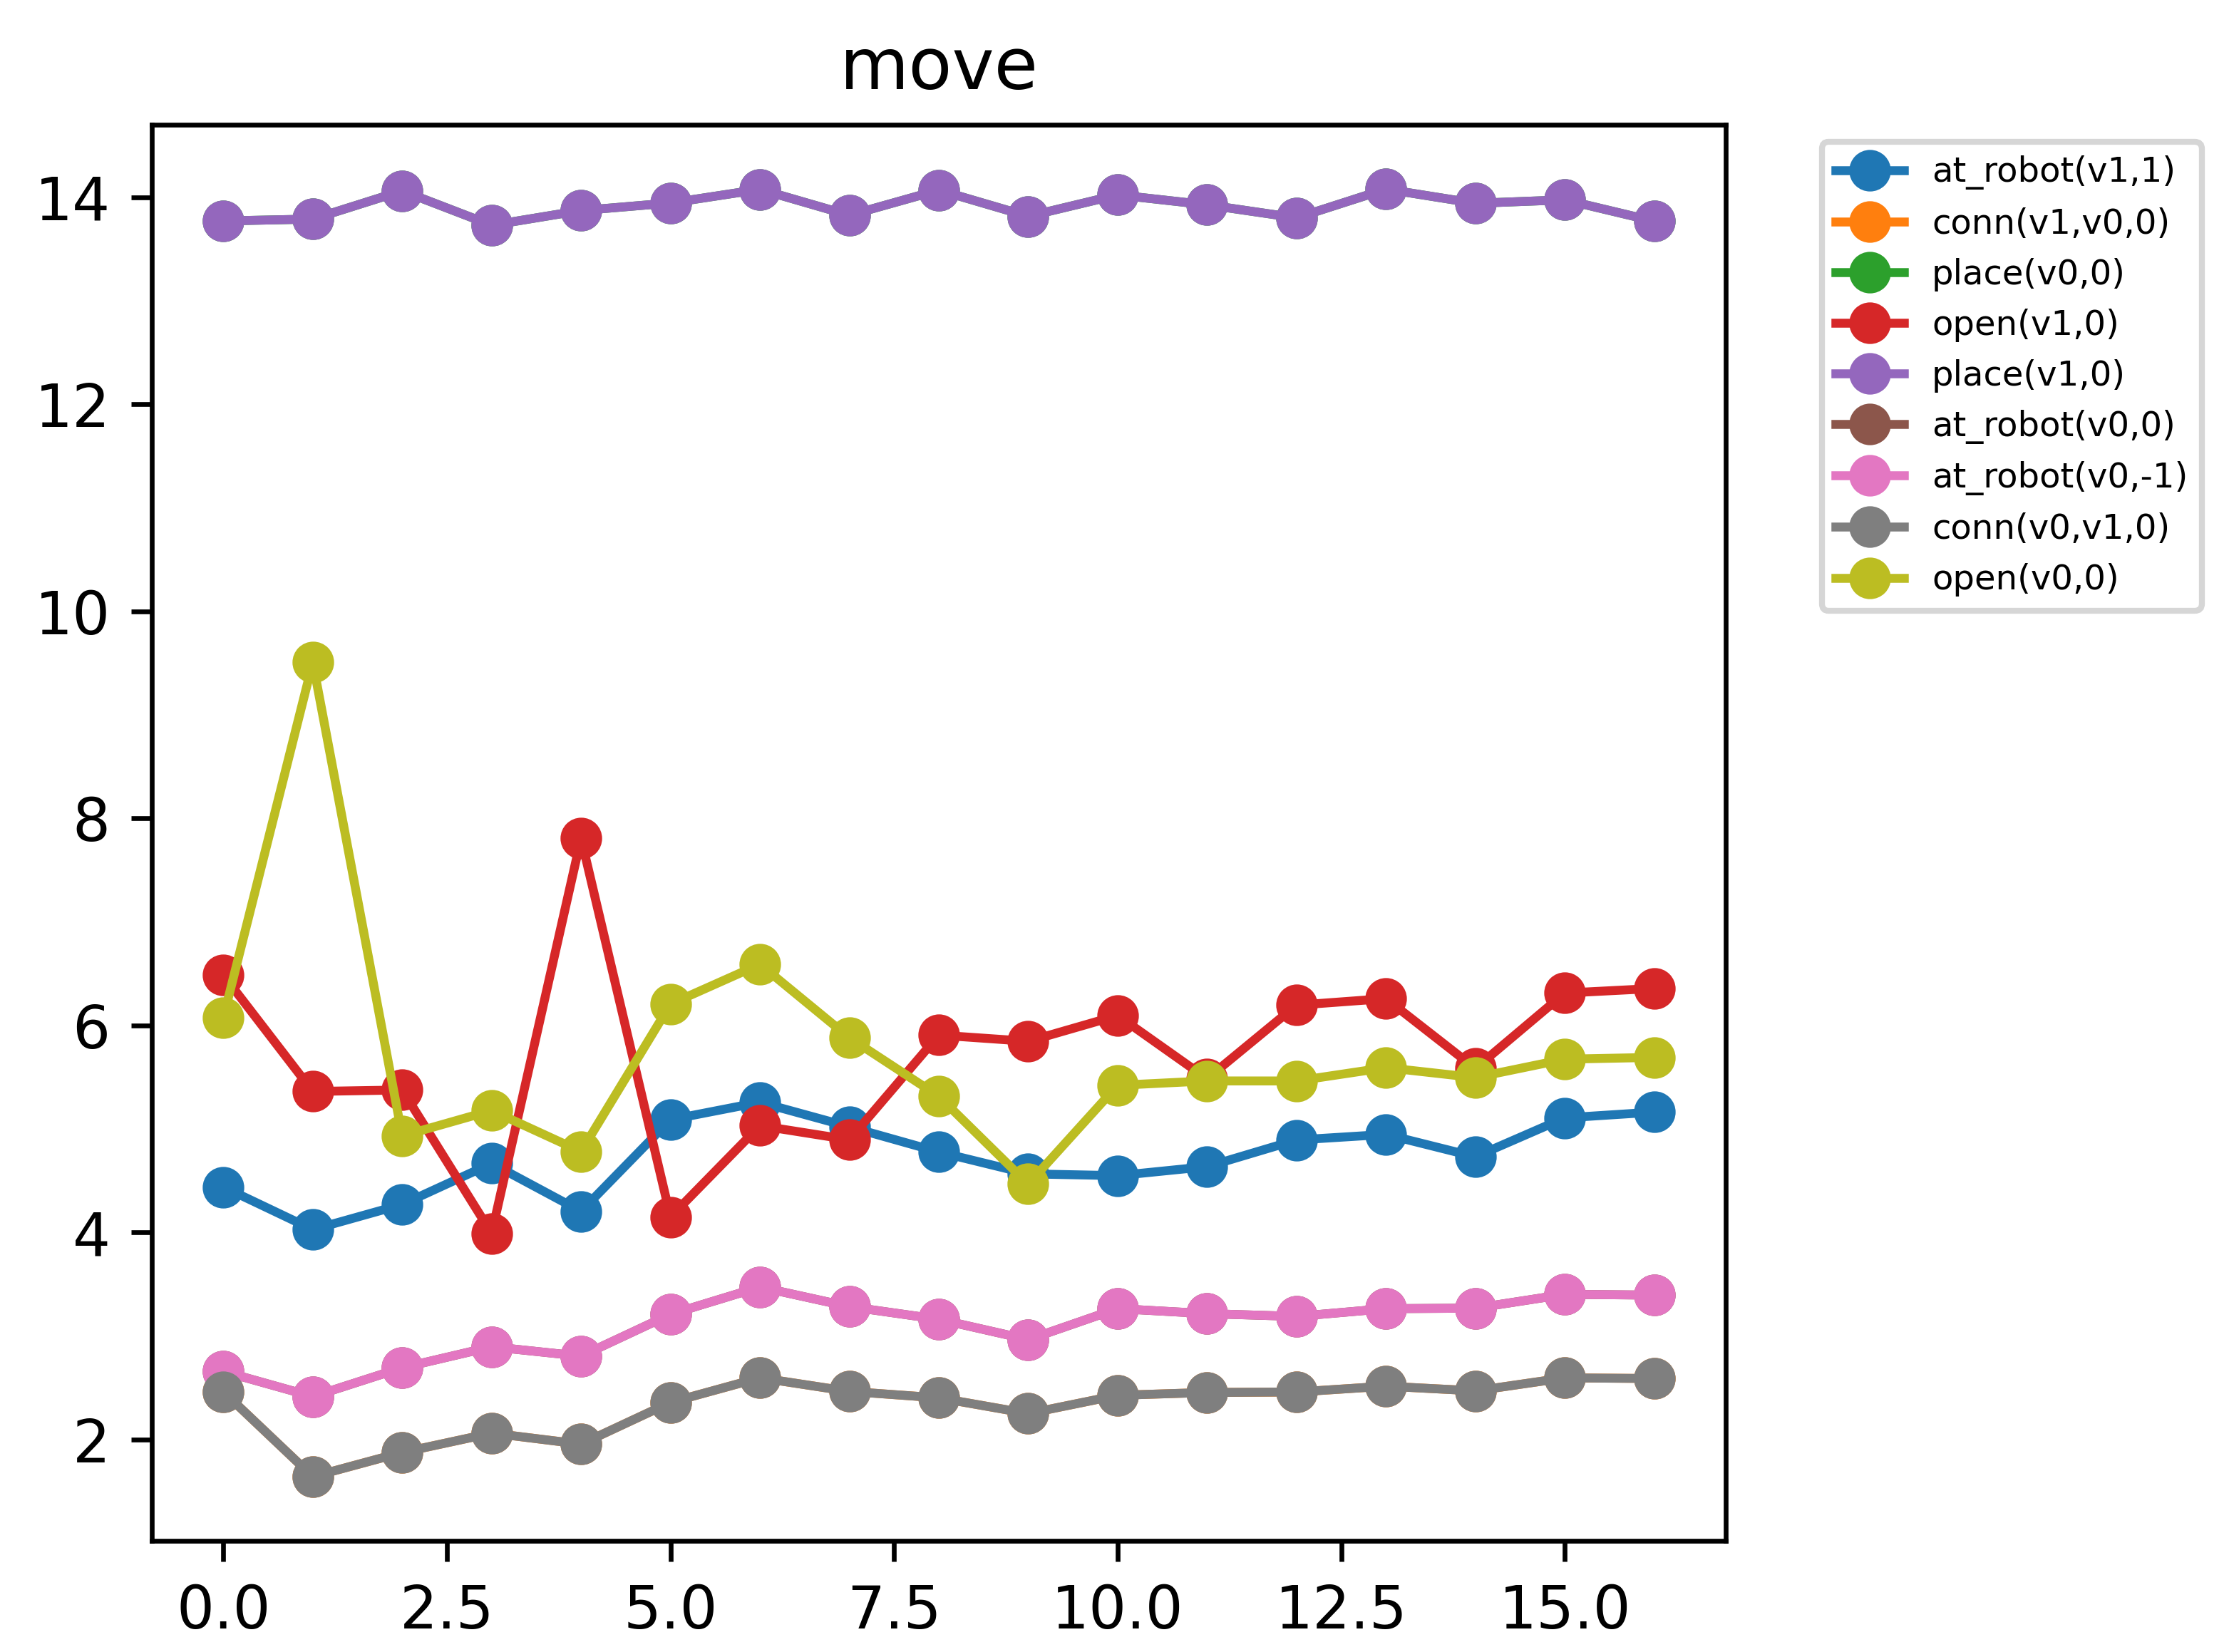
\includegraphics[width=1\textwidth]{images/tests/movegraph_100}
 \caption{Move action MLN, no noise {fig:mv 100}}

 \end{minipage}
 \hfill
 \begin{minipage}[b]{0.49\linewidth}

 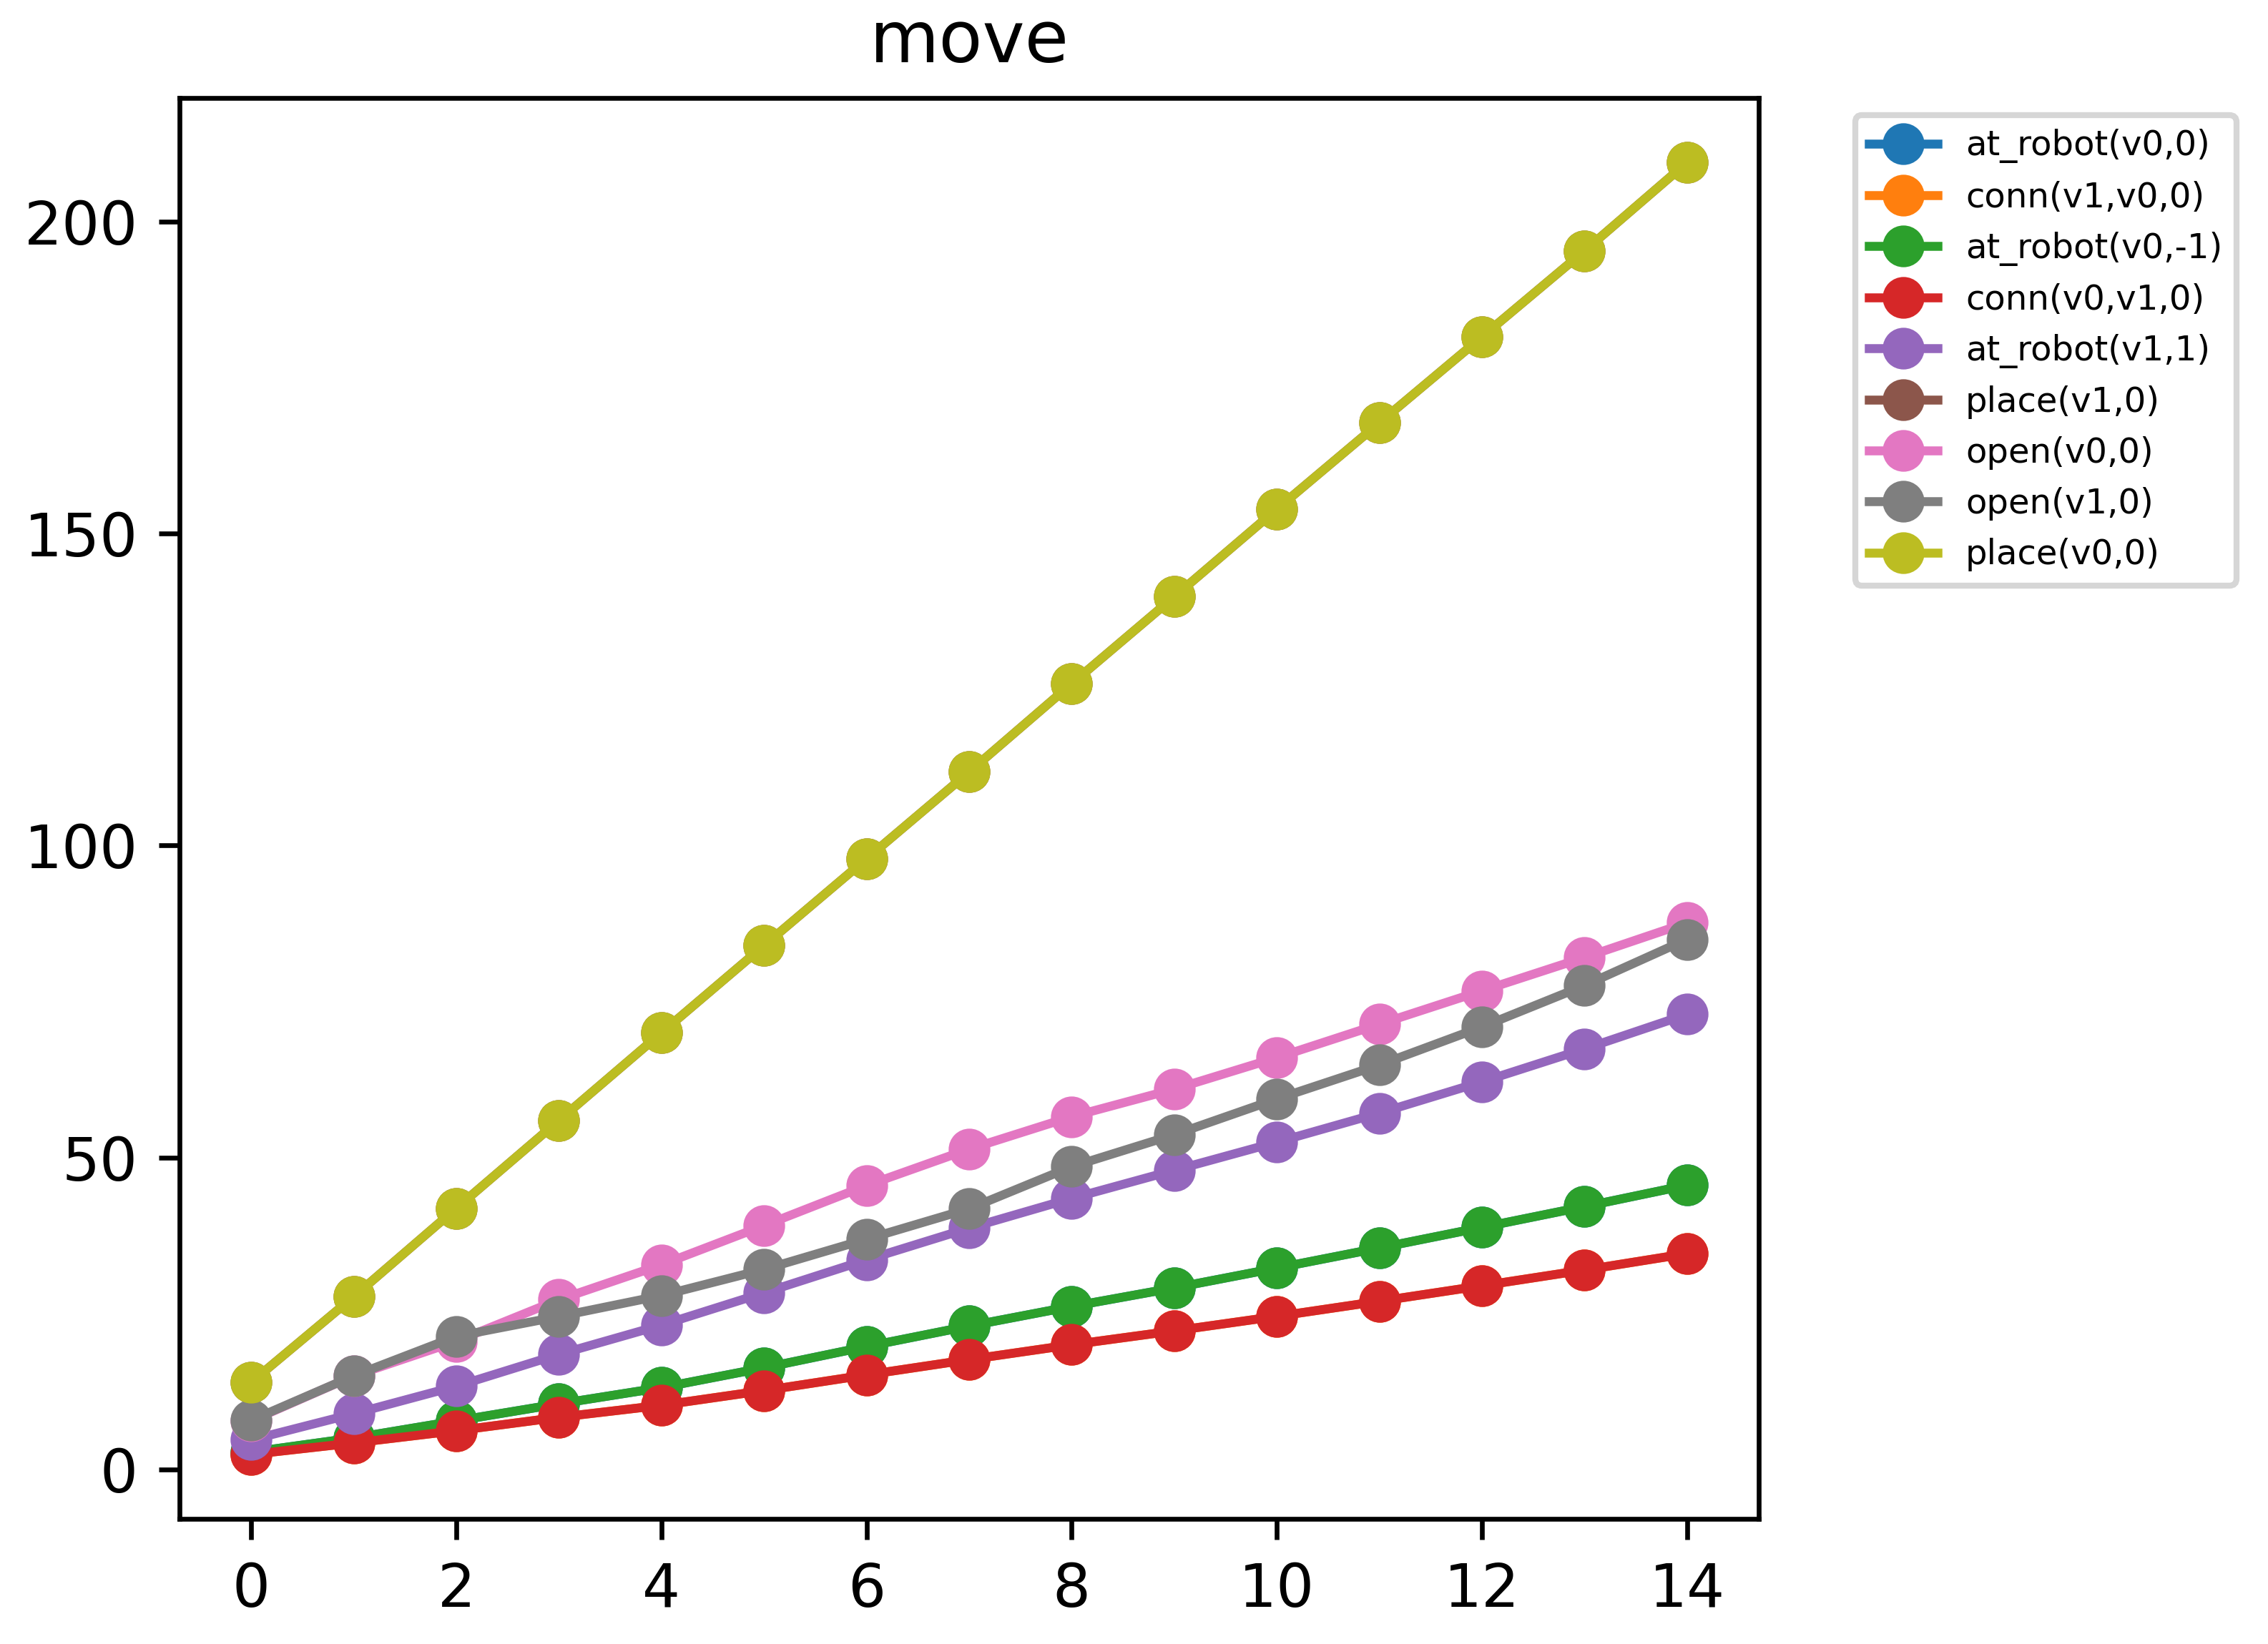
\includegraphics[width=1\textwidth]{images/tests/movegraph_100_cum}
 \caption{Move action MLN (cumulative), no noise {fig:mv 100 cum}}

 \end{minipage}
\end{figure}

As each predicate is part of the action model, we expect none of the weights to be negative, and all lines in the cumulative graph on the left should have a positive gradient between each iteration.
This experiment was run as a sanity test to ensure that indeed an MLN is being trained as expected which is confirmed by the data produced.

In the next set of experiments we ran the same model on data with now 30\% and 70\% random noise on all predicates.
The expectation in this scenario is that more noise would equate to weights approaching 0.
\begin{figure}[h]
 \centering
 \begin{minipage}[b]{0.49\linewidth}
 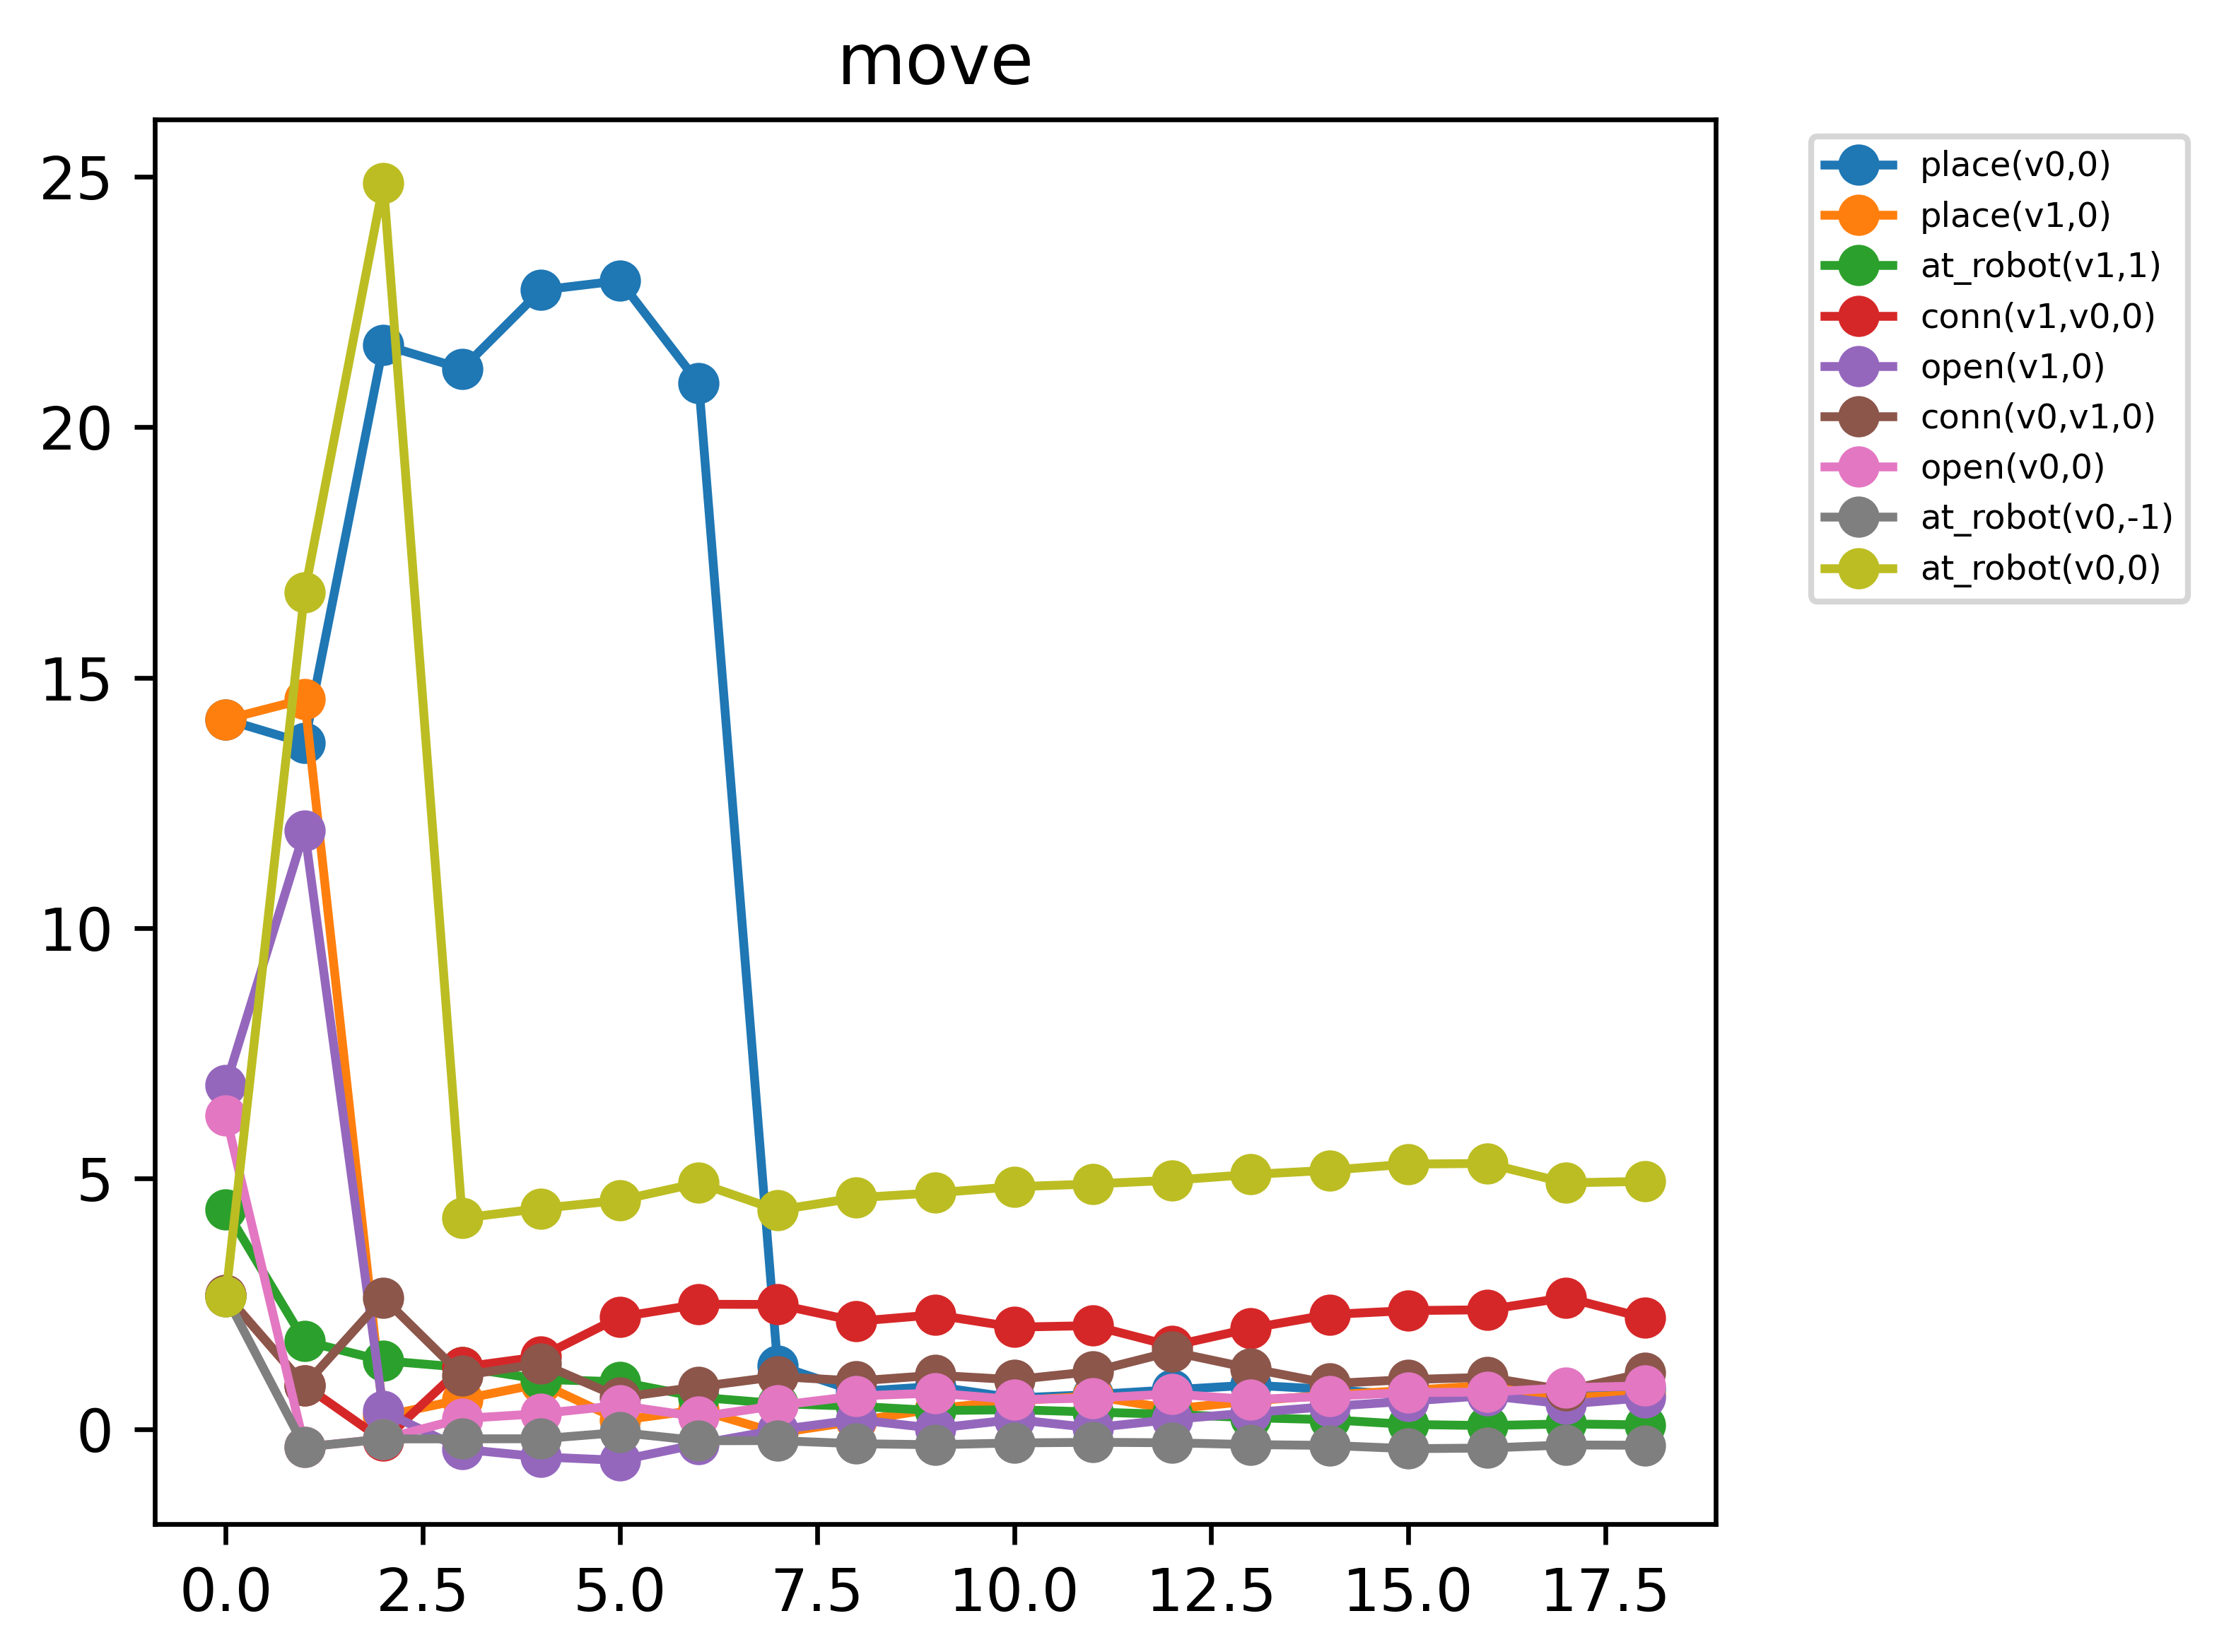
\includegraphics[width=1\textwidth]{images/tests/movegraph_rand_70}
 \caption{Move action MLN, .3 rand noise {fig:mv}}

 \end{minipage}
 \hfill
 \begin{minipage}[b]{0.49\linewidth}

 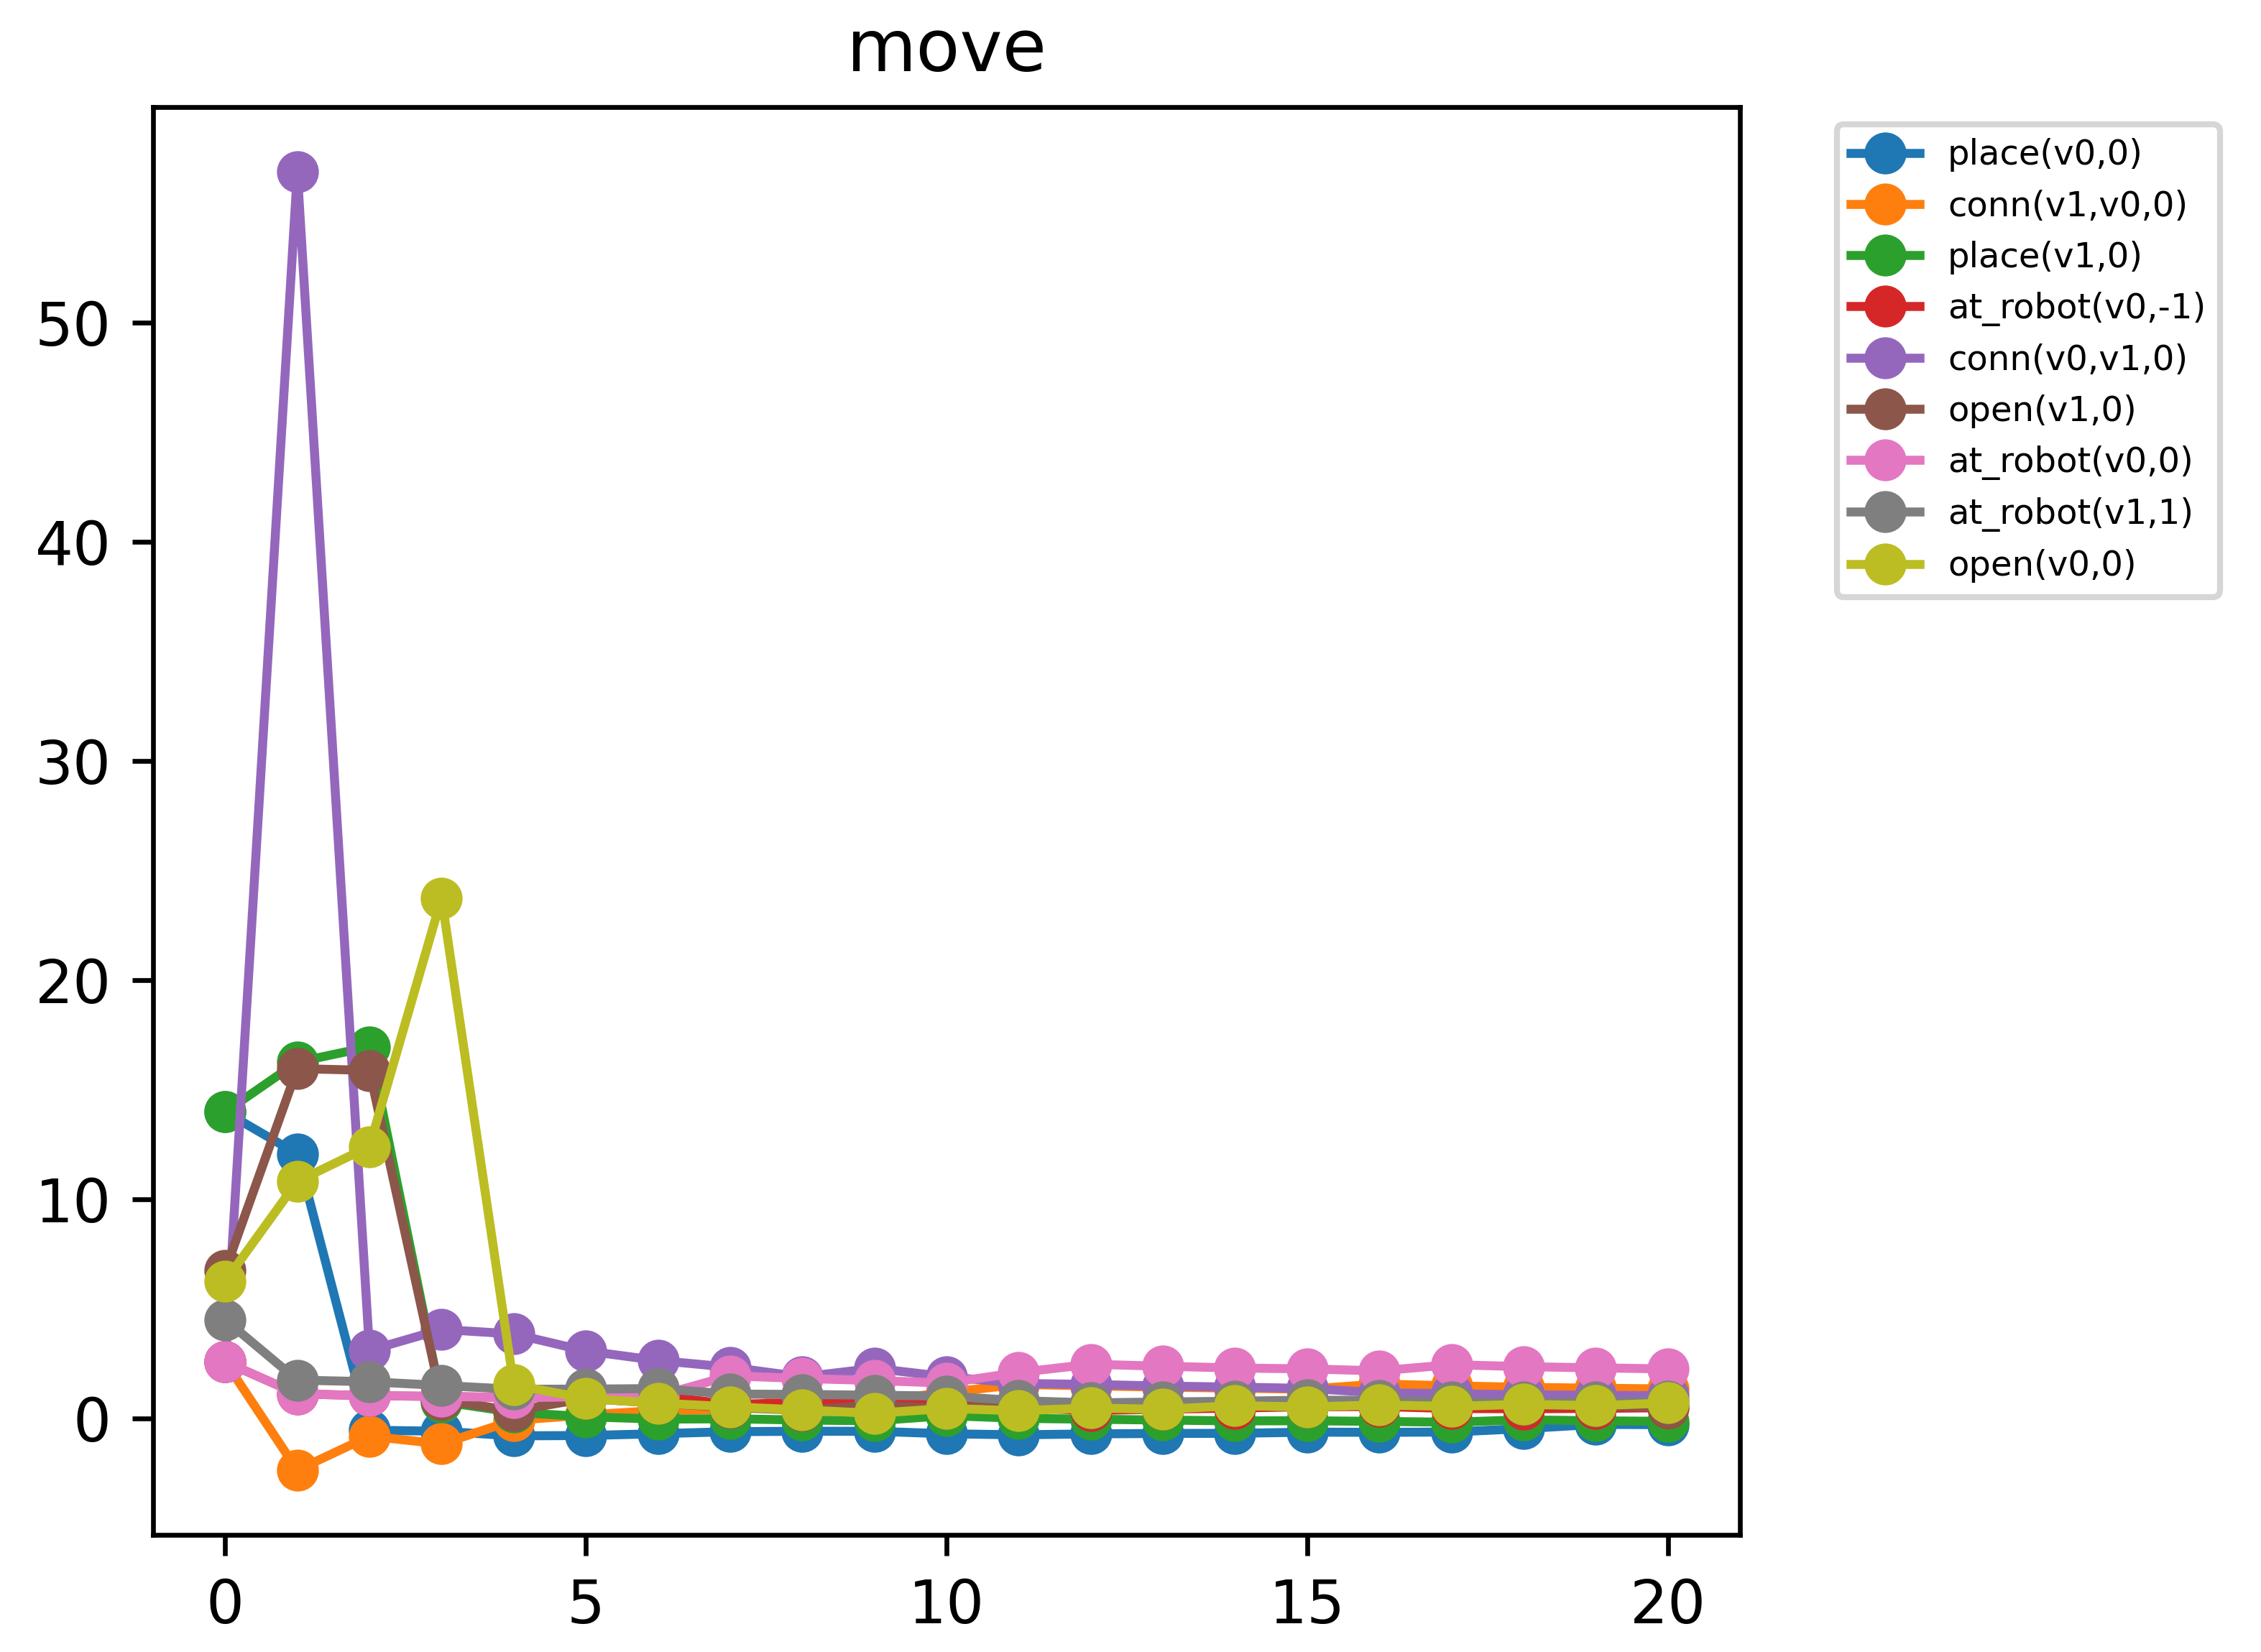
\includegraphics[width=1\textwidth]{images/tests/movegraph_rand_30}
 \caption{Move action MLN, .7 rand noise on){fig:mv 100 cum}}

 \end{minipage}
\end{figure}

The initial spices on some predicates in the above figures, are a result of noise not affecting specific predicates until later iterations, we can see that even with 30\% noise in the dataset weights tend to remain positive, this would be of larger emphasis if predicates not related to the model were included in the training.

Finally we trained the model applying systematic noise to only one predicate, this would be a more common scenario in a real world environment as typically few sensors fail.
The systematic noise is applied on the "conn(v0,v1,0)" predicate.
\begin{figure}[h]
 \centering
 \begin{minipage}[b]{0.49\linewidth}
 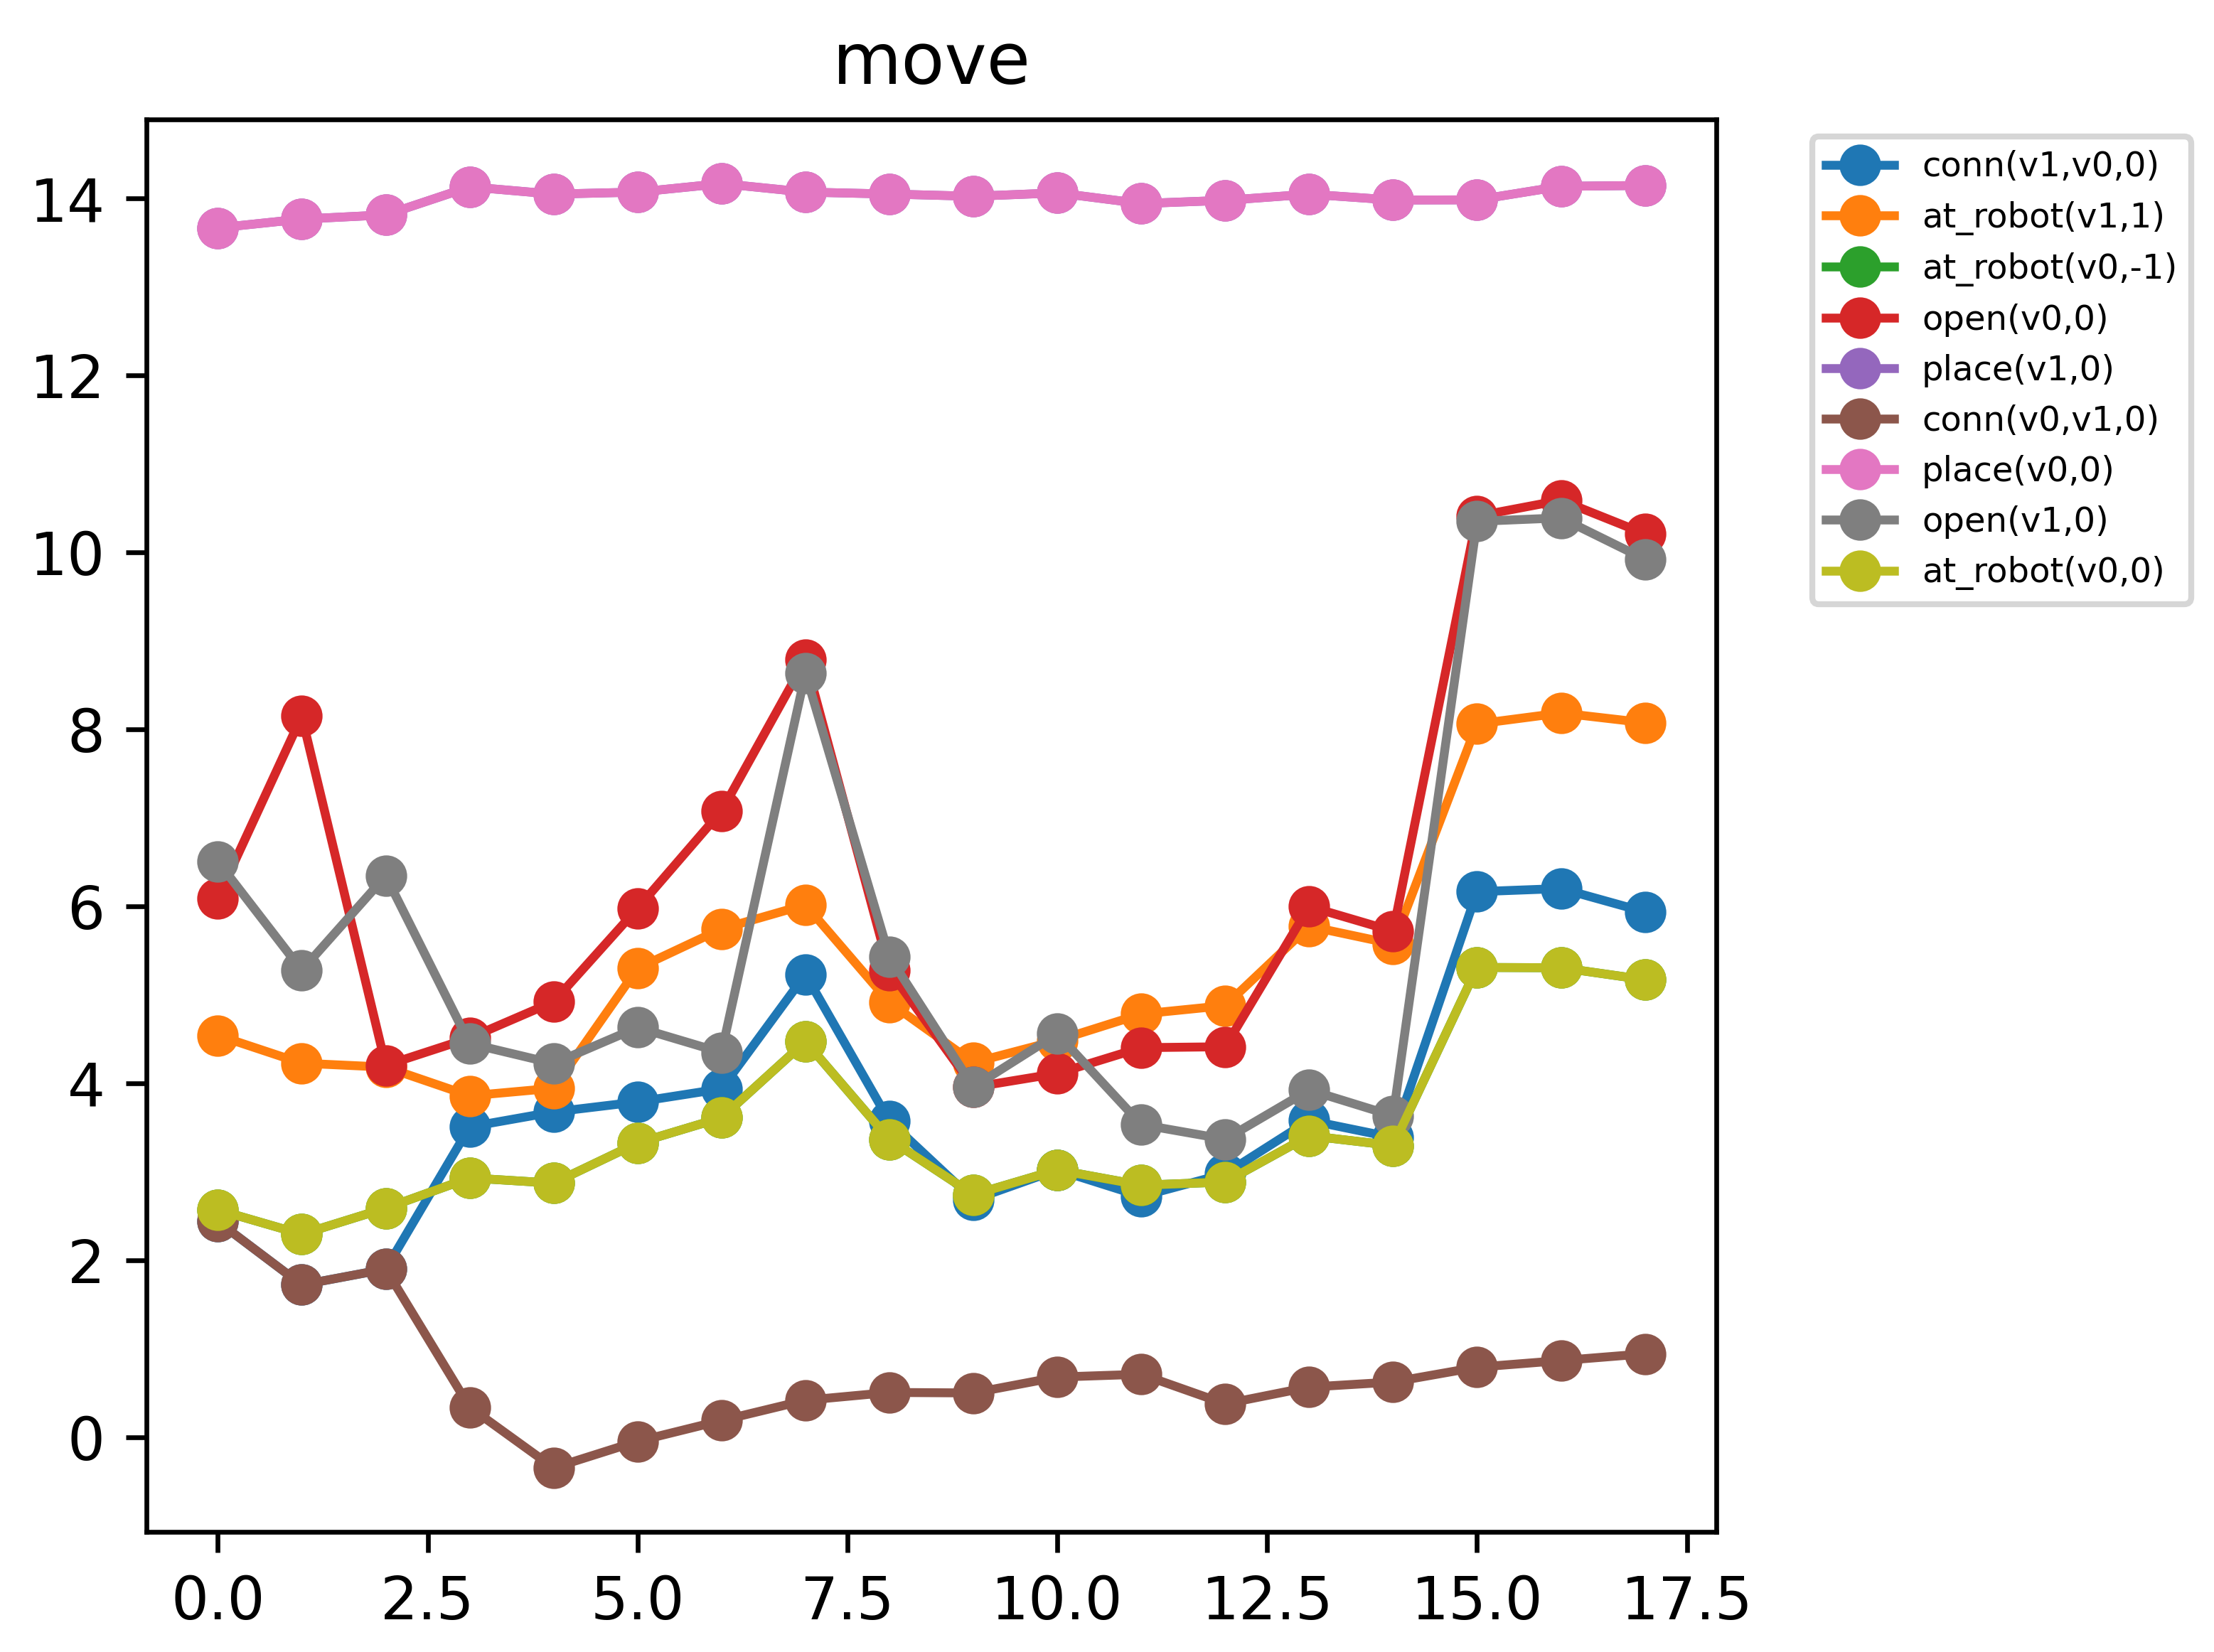
\includegraphics[width=1\textwidth]{images/tests/movegraph_sys_70}
 \caption{Move action MLN, .3 sys noise on conn(v0,v1,0) {fig:mv 100}}

 \end{minipage}
 \hfill
 \begin{minipage}[b]{0.49\linewidth}

 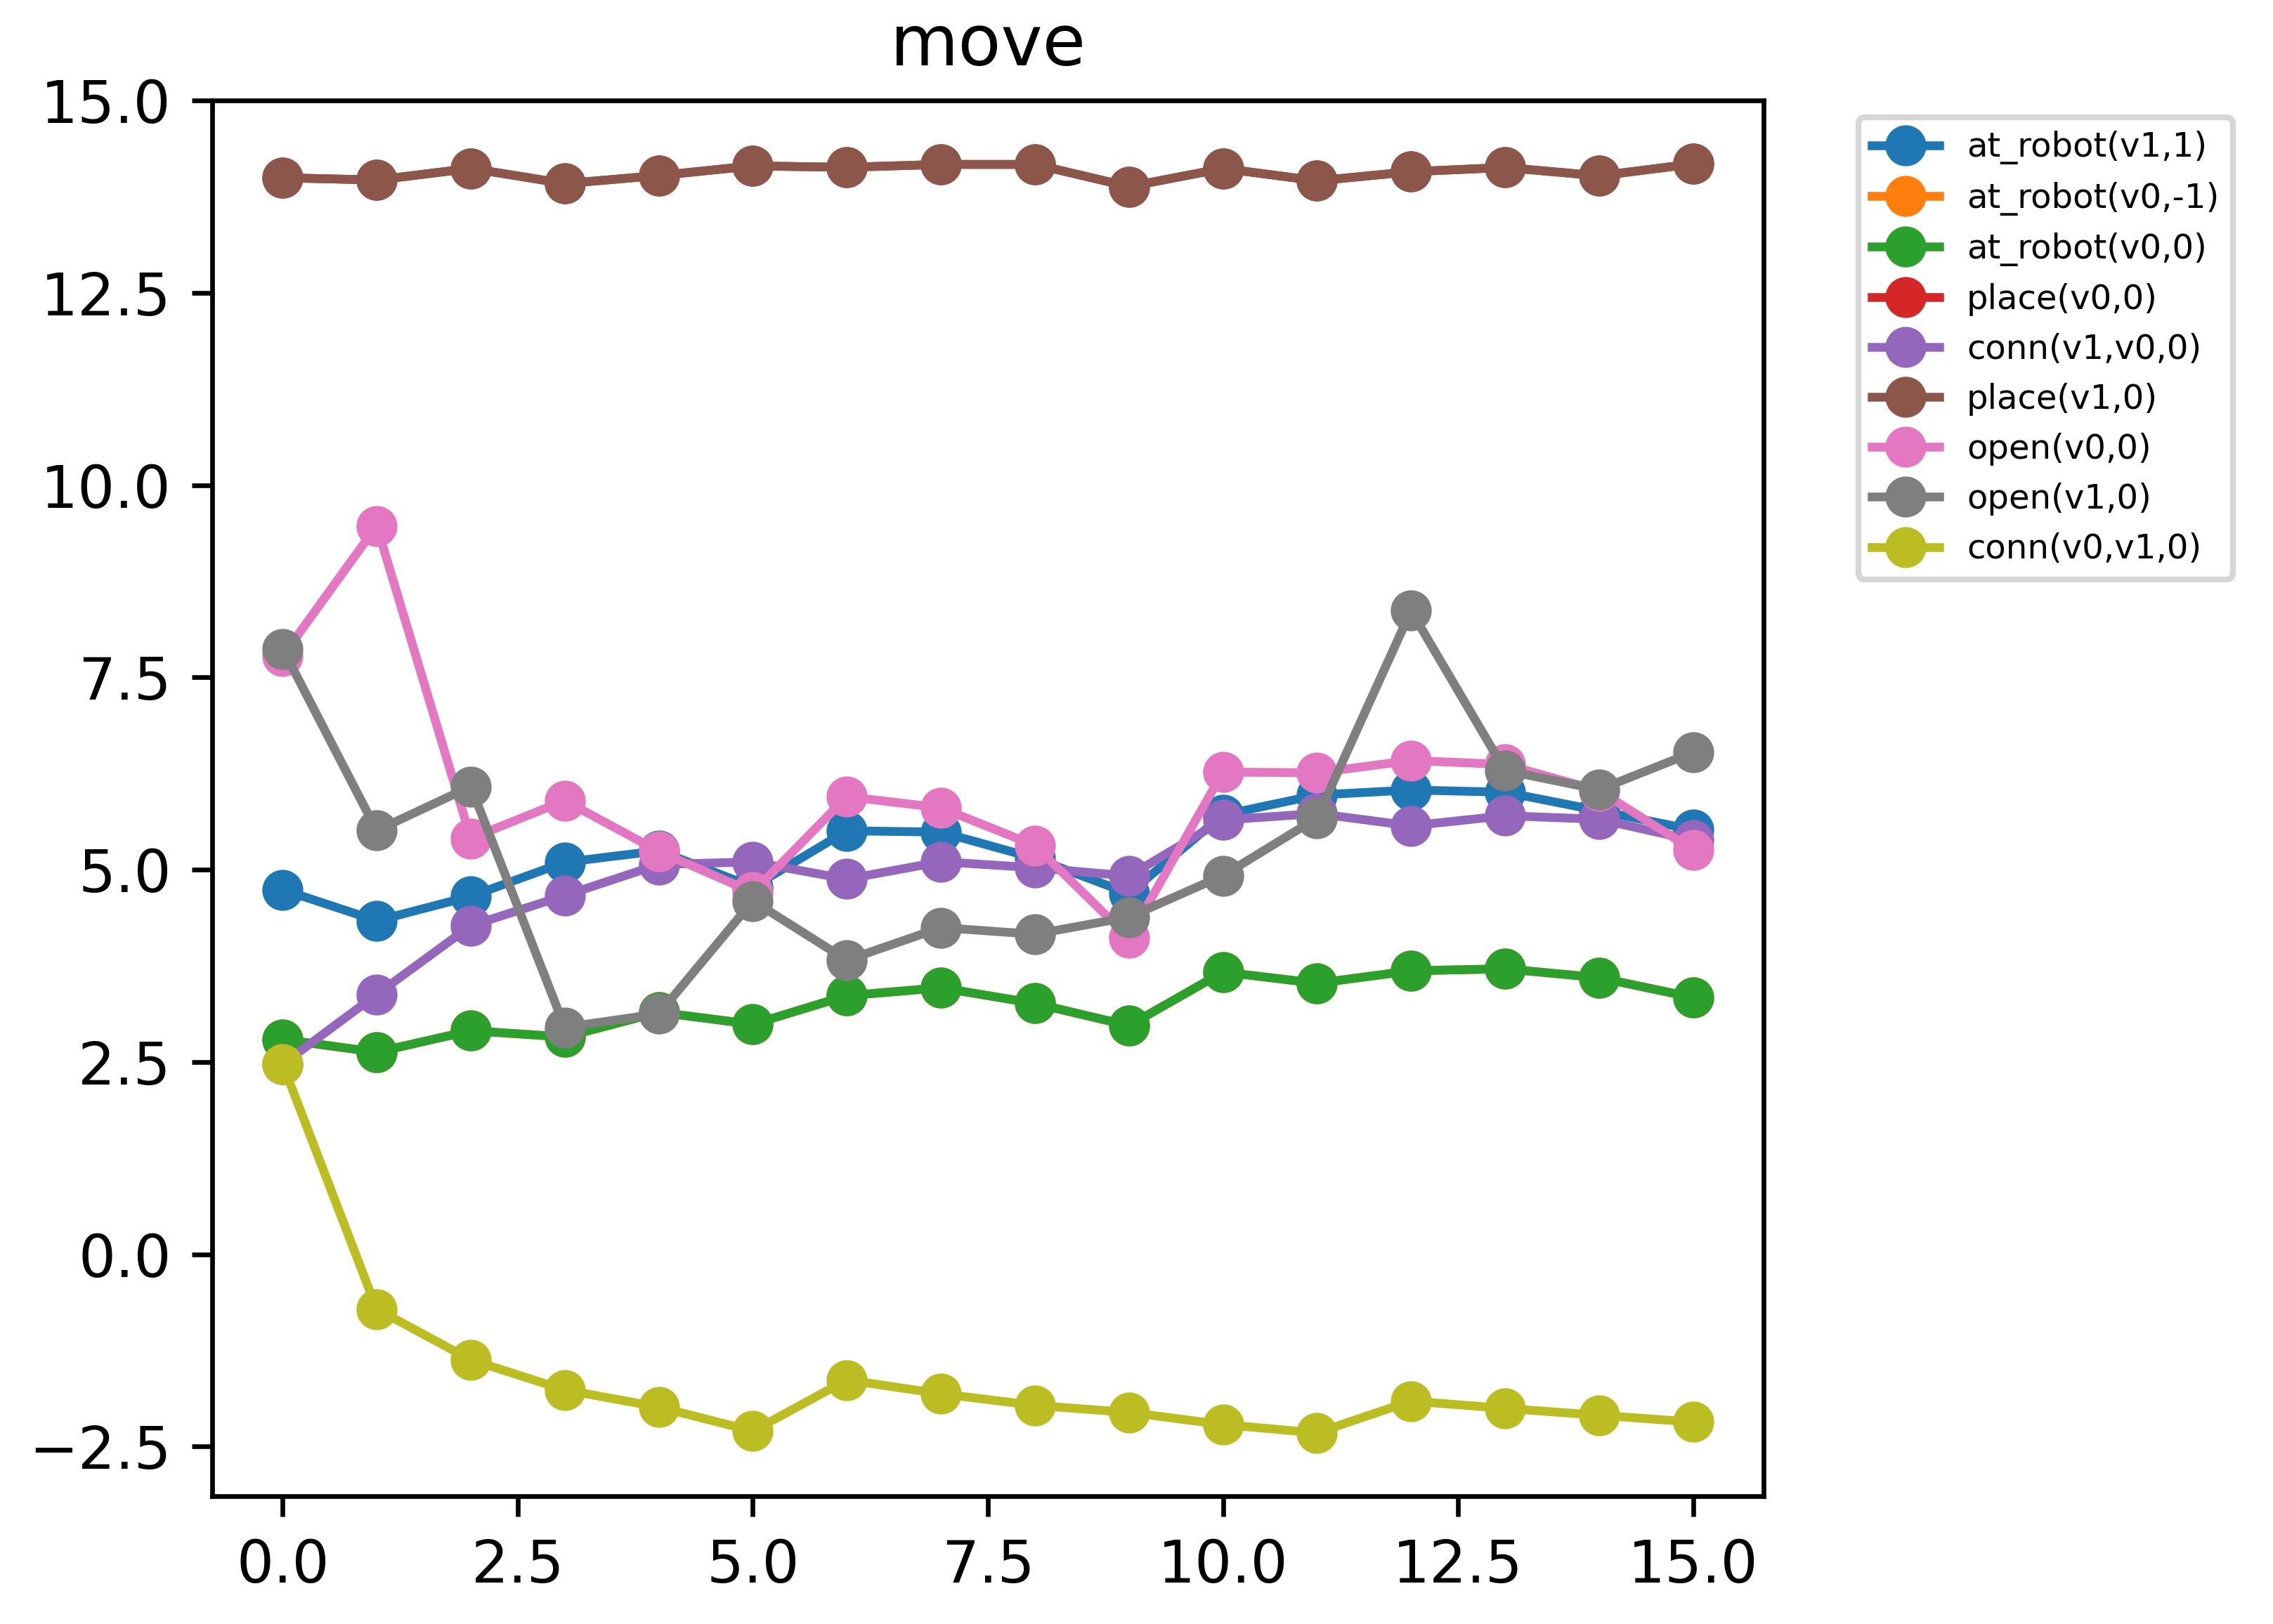
\includegraphics[width=1\textwidth]{images/tests/movegraph_sys_30}
 \caption{Move action MLN, .7 sys noise on conn(v0,v1,0){fig:mv 100 cum}}

 \end{minipage}
\end{figure}

We can observe that systematic noise causes the weights to be pushed down compared to other predicates, however the fact that values are not deeply negative demonstrates the robustness of the model when noise is applied.

The greatest issue with this approach is not the viability of the technique but the efficiency of it.
To train 25 database containing multiple actions, it takes around 30s to 1min, a multicore approach was not implemented in the pracmln package used for training, and a multitude of optimizations and fixes were done in order to speed up training such as patching errors, optimizing data structures and operations over arrays, fixing improperly handled exceptions.
A patched package has been uploaded to the project.
A partial rewrite of the package for training MLN's online is required in order to use this technique on any moderately serious domains (>20 predicates).
Optimizations include multithreading the training process, optimizing operation over grounded predicates and weights.

The results in the figures provided were created by training MLN's on pruned weights as forgoing this step made training impossible.
Training speed reduces significantly when the number of weights are doubled or tripled which is a common occurrence in a normal domain.